\begin{center}
    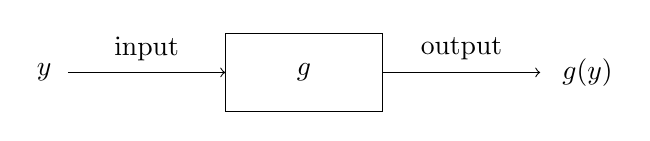
\begin{tikzpicture}
        \draw (0,0.5) rectangle (2,1.5);
        \node at (1,1) {$g$};
        \node at (-2.3, 1) {$y$};
        \node at (4.6, 1) {$g(y)$};
        \draw[->] (-2,1) -- (0,1);
        \draw[->] (2,1) -- (4,1);
        \node at (-1, 1.3) {input};
        \node at (3, 1.3) {output};
    \end{tikzpicture}
    
    \emph{The typical picture one uses when describing a function.}
\end{center}